\documentclass[]{article}

\usepackage{tikz}
\usetikzlibrary{shapes}

\definecolor{red}{RGB}{255,0,0}
\definecolor{green}{RGB}{0, 102, 0}
\definecolor{orange}{RGB}{255,128,0}

\begin{document}

\begin{figure}[h!]
	\centering
	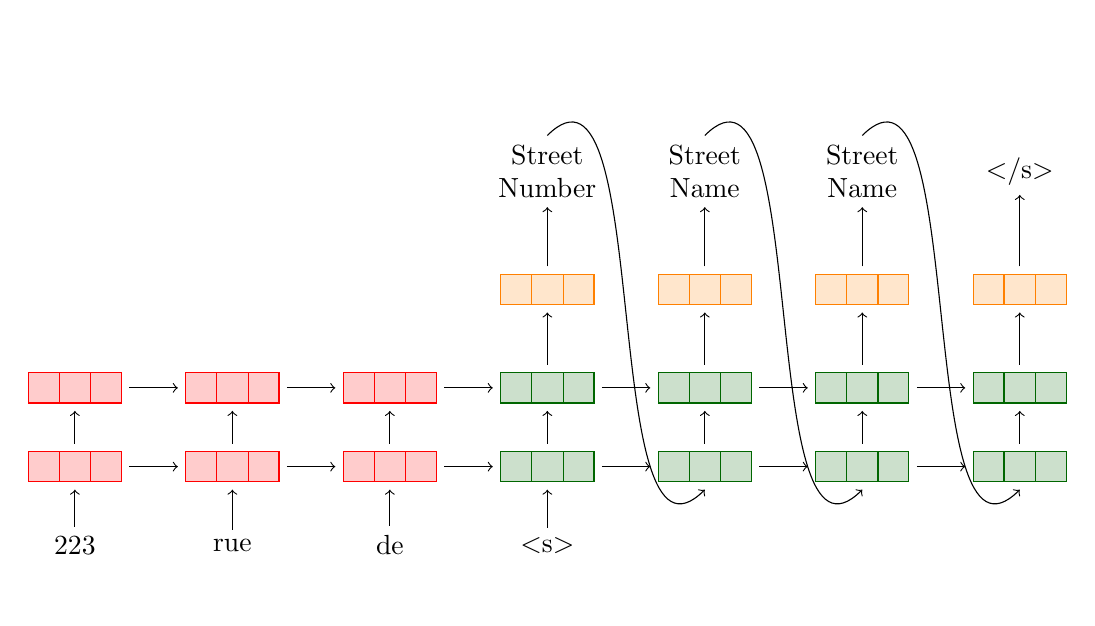
\begin{tikzpicture}[
	hid/.style 2 args={
		rectangle split,
		rectangle split horizontal,
		draw=#2,
		rectangle split parts=#1,
		fill=#2!20,
		outer sep=1mm}, scale=1, every node/.style={scale=1}]
	% draw input nodes
	\foreach \i [count=\step from 1] in {223, rue, de, {{$<$s$>$}}}
	\node (i\step) at (2*\step, -2) {\i};
	% draw output nodes
	\foreach \t [count=\step from 4] in {Street\\Number, Street\\Name, Street\\Name,{{$<$/s$>$}}} {
		\node[align=center] (o\step) at (2*\step, +2.75) {\t};
	}
	% draw embedding and hidden layers for text input
	\foreach \step in {1,...,3} {
		\node[hid={3}{red}] (h\step) at (2*\step, 0) {};
		\node[hid={3}{red}] (e\step) at (2*\step, -1) {};    
		\draw[->] (i\step.north) -> (e\step.south);
		\draw[->] (e\step.north) -> (h\step.south);
	}
	% draw embedding and hidden layers for label input
	\foreach \step in {4,...,7} {
		\node[hid={3}{orange}] (s\step) at (2*\step, 1.25) {};
		\node[hid={3}{green}] (h\step) at (2*\step, 0) {};
		\node[hid={3}{green}] (e\step) at (2*\step, -1) {};    
		\draw[->] (e\step.north) -> (h\step.south);
		\draw[->] (h\step.north) -> (s\step.south);
		\draw[->] (s\step.north) -> (o\step.south);
	}  
	% edge case: draw edge for special input token
	\draw[->] (i4.north) -> (e4.south);
	% draw recurrent links
	\foreach \step in {1,...,6} {
		\pgfmathtruncatemacro{\next}{add(\step,1)}
		\draw[->] (h\step.east) -> (h\next.west);
		\draw[->] (e\step.east) -> (e\next.west);
	}
	% draw predicted-labels-as-inputs links
	\foreach \step in {4,...,6} {
		\pgfmathtruncatemacro{\next}{add(\step,1)}
		\path (o\step.north) edge[->,out=45,in=225] (e\next.south);
	}
	\end{tikzpicture}
	\caption{Seq2seq}\label{fig:seq2seq}
\end{figure}

\end{document}
